%%
\section{Introduction}

The study of the associated production of gauge bosons in hadronic collisions has been established as a crucial test of the standard model (SM) by earlier studies at the LHC as well as the Tevatron  \cite{d0zgg,d0zinv,cdfzgam,cmsvgam,cmsvhgam,atlasvgam,atlasww}. The SM predicts these processes precisely, yet persistent tensions in the SM suggest the need for new physics to appear at the \TeV scale. An inclusive study of the \gmet (or ``monophoton'') final state opens up several beyond-the-SM (BSM) possibilities. Examples of BSM processes that could contribute to \gmet production include new interactions that enhance the cross section for $Z\gamma$ production, new particles that decay to $Z\gamma$, and the production of new invisible particles with an associated photon.
In this search, we will be investigating the latter case, specifically exotic Higgs decays and pair production of dark matter.

\subsection{Exotic Higgs}

Supersymmetric extensions of the Standard Model have the appealing feature that they can stabilize the radiative corrections to the Higgs boson mass, while also providing a natural dark matter particle candidate in the form of the lightest-supersymmetric-particle (LSP). 

In this analysis, we search for supersymmetry (SUSY) in low scale SUSY-breaking scenarios ($\sim$ few \TeV), through the decay of the SM-like Higgs boson into supersymmetric particles. In particular, we are searching for the decay of the Higgs into a gravitino ($G$) LSP and a neutralino NLSP ($\chi_{1}^{0}$), which promptly decays into another gravitino and photon~\cite{Petersson:2012dp}. Fig.~\ref{fig:feynman} shows the Feynman diagram for this process.
Since the gravitino is the LSP in this scenario, the final state signature for this search is an energetic, isolated photon and \met.  We focus on the kinematic region $m_{h}/2 < m_{\chi} < m_{h}$, which this final state is particularly sensitive to. For $m_{\chi} < m_{h}/2$ the Higgs boson can decay into two neutralinos,which will then decay into two gravitinos and 2 photons resulting in a diphoton + met final state.

The neutralino in such models will always be in time. The reason is the the higgs-neutralino-gravitino coupling, i.e. the coupling responsible for this exotic higgs decay, depends inversely on the  supersymmetry breaking scale. In order to have a significant branching ratio for this exotic higgs decay, the supersymmetry breaking scale must be very low.In these models the spin 1/2 goldstino is eaten by the spin 3/2 gravitino, becoming its longitudinal component and this way gravitino acquires a mass proportional to ``f / $M_P$'' where $M_P$ is the plank scale $10^{18}$ GeV and $\sqrt{f}$ is the SUSY breaking scale (at around few TeV). Due to this, gravitino is approximately massless ( $10^{-3}$ eV)  and, due to the supersymmetric equivalence theorem \cite{higgs-gravitino-neutralino} one can replace the gravitino with its goldstino component, which makes the decay possible. 

%For $m_{\chi}<m_{h}/2$, the Higgs can decay into one gravitino and one neutralino, the neutralino then decays into a photon and gravitino. This gives rise to a final state of one photon and missing transverse energy (\met).
%Previous CMS searches for low scale supersymmetry in photon final states have focused on the photon(s)+jets+\met, in the regime where the photons are highly energetic and there is signficant \met.

\begin{figure}[hbtp]
\begin{center}
   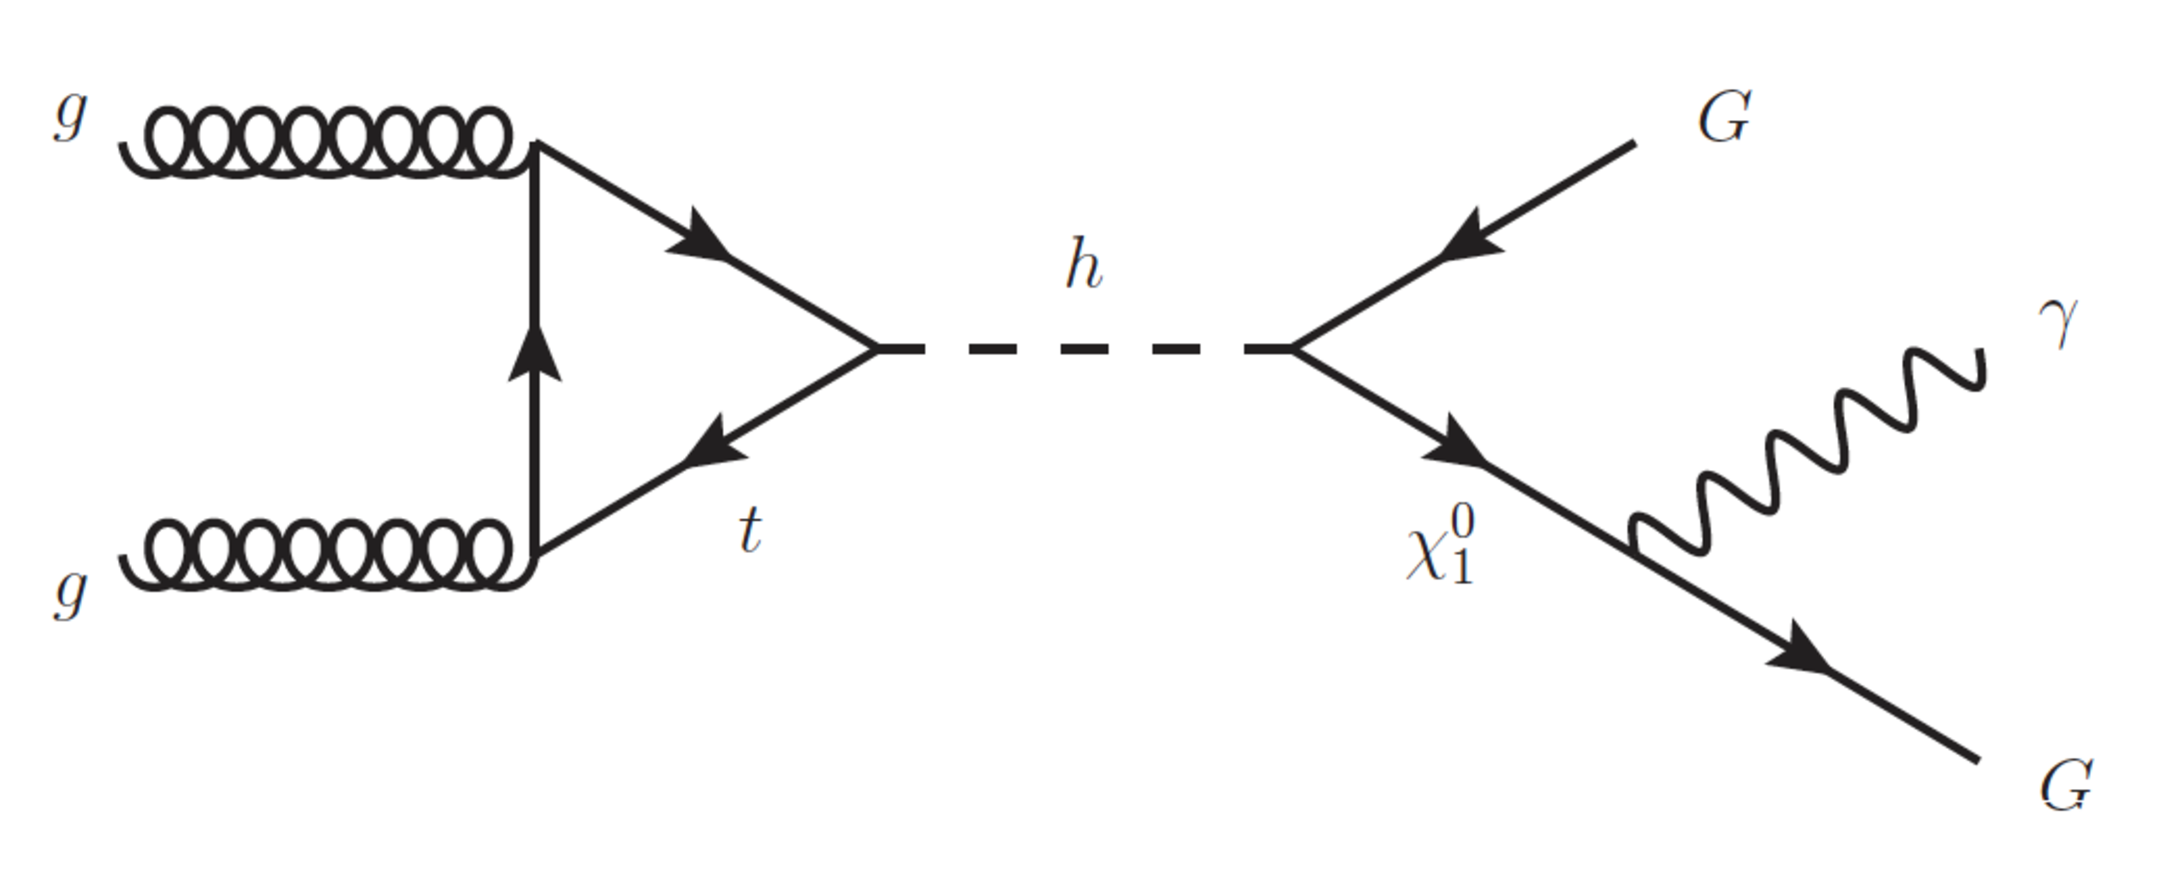
\includegraphics[width=0.6\columnwidth]{analysis_figs/feynman}
 \caption{Feynman diagram of Higgs decay to gravitino (LSP) and a neutralino (NLSP), which subsequently decays to a gravitino and photon. $gg \rightarrow  h \rightarrow  \chi_{1}^{0}  G \rightarrow  \gamma GG$}
 \label{fig:feynman}
\end{center}                                                                                                        
\end{figure} 

\comm{
\subsection{Dark Matter}
The \gmet final state can also be used to set limits on models of dark matter. It is now firmly established that the matter density of the universe is dominated by a non-baryonic dark matter. Searches for a dark matter particle ($D$) take the form of direct detection via elastic scattering off of nuclei or indirect detection via characteristic radiation from $D\overline{D}$ annihilations in astrophysical sources.
At the LHC, this process is accessible via the interaction $q\bar{q} \rightarrow  \gamma D\bar{D}$ where the photon is produced by radiation from the incoming quarks.
The final state in this process consists of a  photon and \met. A similar process can be accessed through the single-jet (monojet) and single-lepton (monolepton) channel ~\cite{Monojet, Monolepton}.

\begin{figure}[hbtp]
\begin{center}
   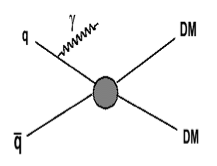
\includegraphics[width=0.3\columnwidth]{analysis_figs/feynDM}
 \caption{Feynman diagrams dark matter production in combination with an ISR photon}
 \label{fig:feynDM}
\end{center}
\end{figure}

Recent theoretical work ~\cite{DMTeva}~\cite{DMLHC} has cast this process in terms of a massive mediator particle ($m_{Med} > 100$~GeV) in the $s$-channel that produces a $D\overline{D}$ pair.
This process is contracted into an effective theory with a contact interaction scale, $\Lambda$, which depends on the mediator mass and its couplings.  The effective operator can be chosen to be either vector or axial-vector, which in turn is used to describe spin-independent or spin-dependent interactions, respectively, as shown below:

\begin{equation}
\mathcal{O}_{\rm V}=\frac{\left(\bar{\chi}\gamma_\mu \chi\right)\left(\bar{q}\gamma^\mu q\right)}{\Lambda^2}
\end{equation}
and
\begin{equation}
\mathcal{O}_{\rm A}=\frac{\left(\bar{\chi}\gamma_\mu \gamma^5 \chi\right)\left(\bar{q}\gamma^\mu \gamma_5 q\right)}{\Lambda^2}
\end{equation}

In the absence of an observed excess of mono-photon events, this  phenomenology can be utilized to establish limits on the effective coupling $\Lambda$. The limits on $\Lambda$ can then be converted to limits on the WIMP-nucleon cross section using the following equations:

\begin{equation}
\sigma_{SI}=\frac{9}{\pi}(\frac{\mu}{\Lambda^2})^2
\end{equation}
and
\begin{equation}
\sigma_{SD}=\frac{0.33}{\pi}(\frac{\mu}{\Lambda^2})^2
\end{equation}
where
\begin{equation}
\mu = \frac{m_{DM} m_p}{m_{DM} + m_p}
\end{equation}

Recent results from the high \pt monophoton search has excluded previously inaccessible DM masses below 3.5 \GeV for a $\chi$-nucleon cross section greater than 0.03 fb at 90\% CL. In this analysis we present complementary results in the more challenging low \pt and low \met region.

%\subsection{Dark Photons}
}